\documentclass[12pt,a4paper,titlepage]{article}


\usepackage[raggedright]{titlesec}
\usepackage[makeroom]{cancel}
\usepackage{amsmath}
\usepackage{amssymb}
\usepackage{graphicx}
\usepackage{hyperref}
\usepackage{listings}
\usepackage{xcolor}
\usepackage[margin=3cm]{geometry}


\lstdefinestyle{scala}{
  frame=tb,
  language=scala,
  aboveskip=3mm,
  belowskip=3mm,
  showstringspaces=false,
  columns=flexible,
  basicstyle={\small\ttfamily},
  numbers=left,
  numberstyle=\tiny\color{gray},
  keywordstyle=\color{blue},
  commentstyle=\color{dkgreen},
  stringstyle=\color{mauve},
  frame=single,
  breaklines=true,
  breakatwhitespace=true,
  tabsize=2,
}

\hypersetup{
  hidelinks,
  colorlinks=false
}

\setlength{\parskip}{1em}


\title{Differential Equations Computational Practicum Report - Variant 12}
\author{Tymur Lysenko}
\date{November, 2019}


\begin{document}
  \pagenumbering{gobble}
  \maketitle
  \tableofcontents
  \newpage
  \pagenumbering{arabic}

  \section{Solution to the provided differential equation} \label{problem}

  Solve the following initial value problem analytically:
  \begin{equation} \label{task_ivp}
    \begin{cases}
      y' = 5 - x^2 - y^2 + 2xy\\
      y(0) = 1 = y(x_0) = y_0
    \end{cases}
  \end{equation}
  The differential equation from the IVP above is a \textbf{Riccati} equation:
  \begin{enumerate}
    \item Find its any non-trivial particular solution $y_1$. Suppose the particular solution is of the form: 
    \begin{equation} \label{par_sol_prop}
      y_1 = c_1 + c_2 x
    \end{equation}
    then
    \begin{equation} \label{par_sol_prop_der}
      y_1' = c_2
    \end{equation}
    Substituting \eqref{par_sol_prop} and \eqref{par_sol_prop_der} into the \eqref{task_ivp} and rearranging the terms yields:
    \begin{equation*}
      c_2 + c_1^2 + 2c_1c_2x + c_2^2 x^2 - 2c_1x - 2c_2 x^2 = 5 - x^2
    \end{equation*}
    Grouping of terms with the corresponding coefficients produces:
    \begin{equation*}
      (c_2^2 - 2c_2)x^2 + 2c_1(c_2 - 1)x + c_1^2 + c_2 = 5 - x^2
    \end{equation*}
    To find $c_1$ and $c_2$ solve the below system of equations follows from the above equation:
    \begin{equation*}
      \begin{cases}
        c_2^2 - 2c_2 = -1\\
        c_2 - 1 = 0\\
        c_1^2 + c_2 = 5
      \end{cases}
      \iff
      \begin{cases}
        c_2 = 1\\
        c_1^2 + 1 = 5\\
        1 - 2 = -1
      \end{cases}
      \iff
      \begin{cases}
        c_1 = \pm 2\\
        c_2 = 1\\
        -1 = -1
      \end{cases}
    \end{equation*}
    Since only 1 solution is enough, let the particular solution of \eqref{task_ivp} be:
    \begin{equation} \label{par_sol}
      y_1 = 2 + x
    \end{equation}

    \item The solution to the Riccati equation has a form:
    \begin{equation} \label{gen_form_sol}
      y = y_1 + u(x) = 2 + x + u, \text{where $u$ is a function of $x$}
    \end{equation}
    So:
    \begin{equation} \label{gen_form_sol_der}
      y' = 1 + u'
    \end{equation}
    \begin{align}
      y^2 &= (2 + x + u)^2 \nonumber \\
      &= 4 + 2x + 2u + 2x + x^2 + ux + 2u + ux + u^2 \nonumber \\
      &= u^2 + 4u + x^2 + 4x + 2ux + 4 \label{gen_form_sol_sq}
    \end{align}
    Substitute \eqref{gen_form_sol}, \eqref{gen_form_sol_der} and \eqref{gen_form_sol_sq} to the \eqref{task_ivp}:
    \begin{equation*}
      \cancel{1} + u' = \cancel{5} - \cancel{x^2} - u^2 - 4u - \cancel{x^2} - \cancel{4x} - \cancel{2ux} - \cancel{4} + \cancel{4x} + \cancel{2x^2} + \cancel{2xu}
    \end{equation*}

    The above equation is a \textbf{Bernoulli} equation, which needs to be solved with respect to $u$:
    \begin{equation} \label{bernoulli}
      u' + 4u = -u^2
    \end{equation}
    \begin{enumerate}
      \item Solve the complementary equation to the \eqref{bernoulli}:
      \begin{gather*}
        u'_c = -4u_c\\
        \int \frac{du_c}{u_c} = -4 \int dx, u_c \neq 0\\
        ln|u_c| = -4x + c_3\\
        u_c = c_4e^{-4x}
      \end{gather*}
      Since it is enough to have any solution to the complementary equation to solve the \eqref{bernoulli}, for simplicity take $c_4 = 1$, so:
      \begin{equation} \label{bernoulli_comp_sol}
        u_c = e^{-4x}
      \end{equation}

      \item Use \eqref{bernoulli_comp_sol} to find $u$ by variating the parameter $v$:
      \begin{equation} \label{u}
        u = u_cv = \frac{v}{e^{4x}} \text{, where $v$ is a function of $x$}
      \end{equation}
      \begin{equation} \label{u'}
        u' = \frac{e^{4x}v' - 4e^{4x}v}{e^{8x}}
      \end{equation}
      \begin{equation} \label{u_sq}
        u^2 = \frac{v^2}{e^{8x}}
      \end{equation}
      Substitute \eqref{u}, \eqref{u'} and \eqref{u_sq} into the \eqref{bernoulli} to find $v$:
      \begin{equation*}
        \frac{e^{4x}v' - 4e^{4x}v}{e^{8x}} + 4\frac{v}{e^{4x}} = -\frac{v^2}{e^{8x}}
      \end{equation*}
      Multiply both sides by $e^{8x}$:
      \begin{gather*}
        e^{4x}v' - \cancel{4e^{4x}v} + \cancel{4e^{4x}v} = v^2\\
        v' = -\frac{v^2}{e^{4x}}
      \end{gather*}
      Solve the above \textbf{separable} differential equation with respect to $v$:
      \begin{gather}
        \int \frac{dv}{v^2} = - \int e^{-4x} dx \nonumber \\
        - \frac{1}{v} = \frac{1}{4}e^{-4x} + c \nonumber \\
        v = \frac{4}{c - e^{-4x}} \label{v}
      \end{gather}
      The \eqref{v} can now be substituted to \eqref{u}, which is the most general solution for \eqref{bernoulli}:
      \begin{equation} \label{bernoulli_sol}
        u = \frac{4}{ce^{4x} - 1}
      \end{equation}
    \end{enumerate}

    Now it is possible to get back to \eqref{gen_form_sol} and write \textbf{the most general solution for the differential equation from the IVP \eqref{task_ivp}}, by substituting $u$ with \eqref{bernoulli_sol}:
    \begin{equation} \label{ivp_de_sol}
      y = 2 + x + \frac{4}{ce^{4x} - 1}
    \end{equation}

    The \eqref{ivp_de_sol} is \textit{undefined}, when:
    \begin{gather*}
      ce^{4x} = 1 \\
      e^{4x} = \frac{1}{c}
    \end{gather*}
    \begin{equation} \label{undefined_point}
      x = \frac{ln(\frac{1}{c})}{4}
    \end{equation}

    \item To finish solving the initial value problem \eqref{task_ivp} express the general formula for $c$ in terms of the initial condition $y_0$ and $x_0$ and the substitute the given corresponding values:
    \begin{gather*}
      y_0 - 2 - x_0 = \frac{4}{ce^{4x_0} - 1} \\
      ce^{4x_0} - 1 = \frac{4}{y_0 - 2 - x_0}
    \end{gather*}
    \begin{equation} \label{gen_c}
      c = \frac{2 + y_0 - x_0}{e^{4x_0}(y_0 - x_0 - 2)}
    \end{equation}
    \begin{equation} \label{c}
      c = \frac{2 + 1 - 0}{e^{4*0}(1 - 0 - 2)} = \frac{3}{1*(-1)} = -3
    \end{equation}
    From \eqref{gen_c} it follows that the IVP \eqref{task_ivp} is not solvable, when the initial condition satisfies the equation:
    \begin{equation}
      y_0 = x_0 + 2
    \end{equation}

    So, \textbf{the solution to the IVP \eqref{task_ivp}} is:
    \begin{equation} \label{ivp_sol}
      y = 2 + x - \frac{4}{3e^{4x} + 1}
    \end{equation}
    Because of the \eqref{undefined_point} and \eqref{c} the solution \eqref{ivp_sol} is defined $\forall x \in \mathbb{R}$.
  \end{enumerate}


  \newpage
  \section{Application demonstration}

  \subsection{General description}

  The application's source code is available on Github: \url{https://github.com/TymurLysenkoIU/DE}

  The application is implemented in \textbf{Scala.js} with the use of \textbf{Binging.scala} for UI and \textbf{Plotly.js} for plotting graphs. It implements the:
  \begin{itemize}
    \item \textbf{Euler}
    \item \textbf{improved Euler}
    \item \textbf{Runge-Kutta}
  \end{itemize}
  numerical methods and applies the to the IVP from the section \ref{problem}. As the result, it plots the calculated values of the \textit{solution}, \textit{local truncation error} and \textit{maximal local truncation error} for the specified interval of number of intervals.

  UML diagram of the application generated by IntelliJ IDEA can be found in the \textbf{./img/class-uml-diagram.png}.

  \newpage
  \subsection{UI}

  \begin{figure}[h!]
    \centering
    \frame{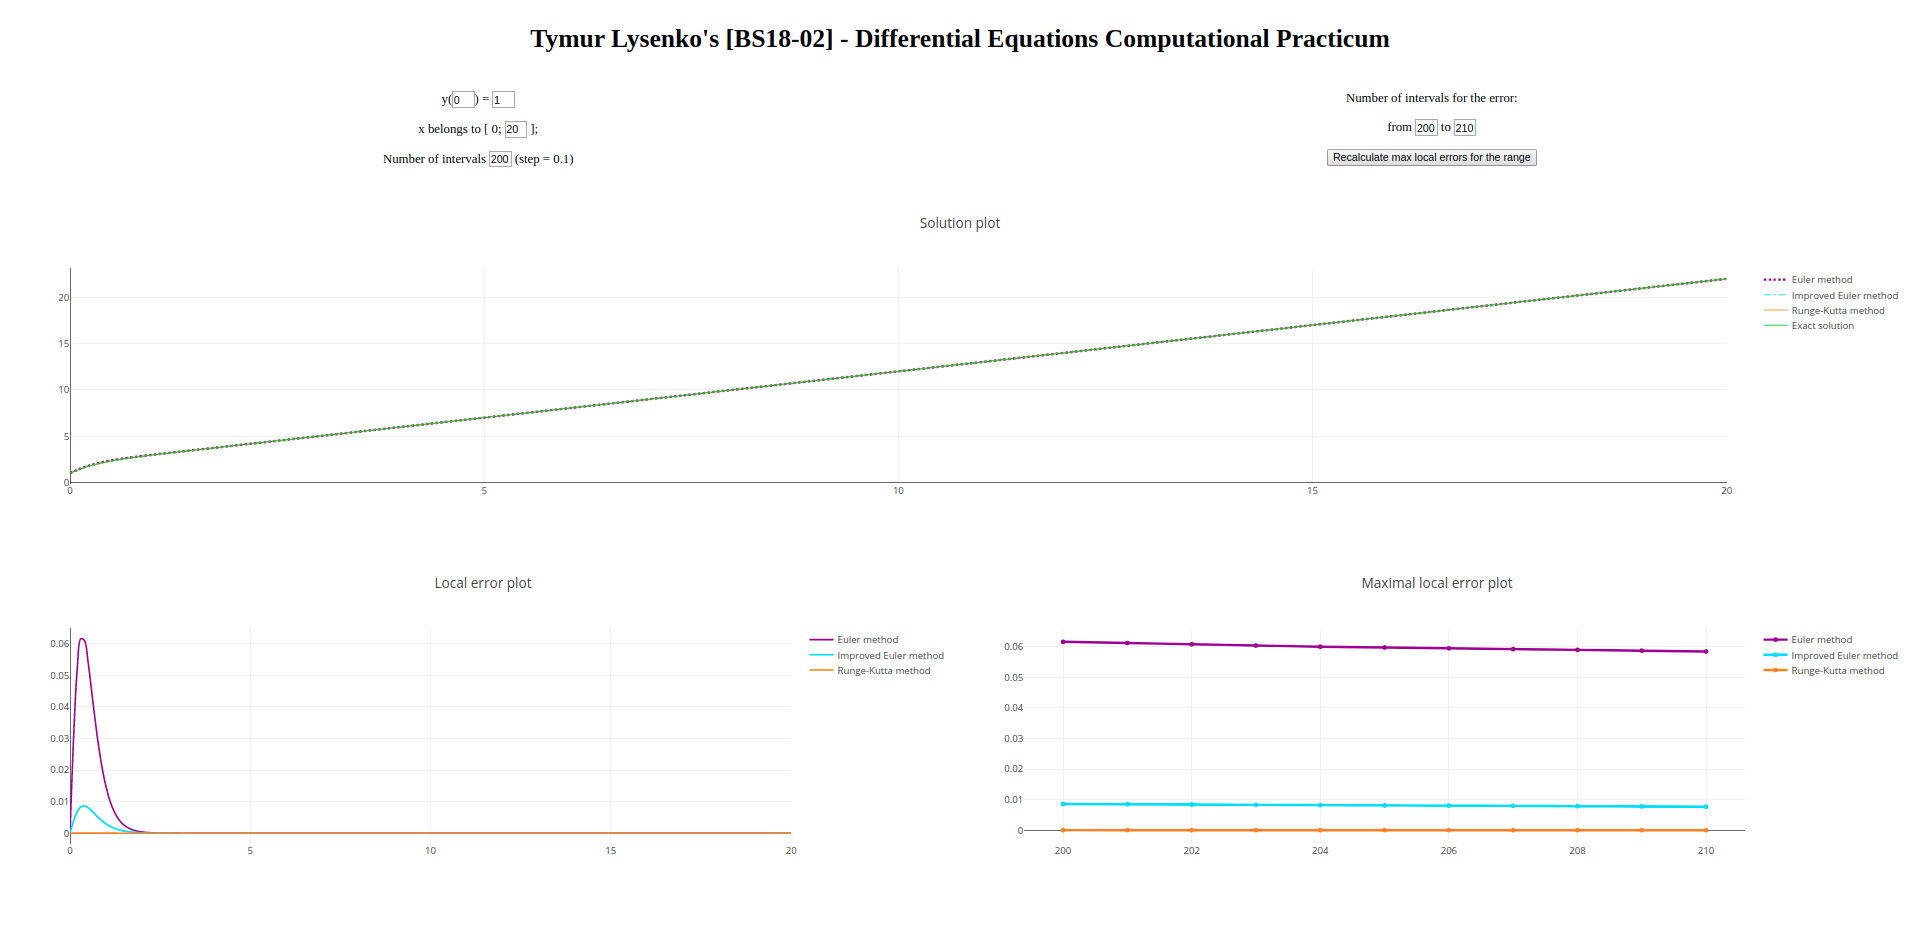
\includegraphics[width=\linewidth]{img/application_ui.png}}
    \caption{Application UI}
  \end{figure}

  The above figure demonstrates the UI of the implemented application. The application enables to input the \textit{initial conditions for the IVP}, \textit{interval that $x$ belongs to} and a \textit{number of intervals} (which affect the step). The application reacts to changes of these values and redraws the \textit{solution} and \textit{local error} plots.

  The UI also allows specifying the \textit{interval for the number of intervals}. The application does not react to changes the interval, instead, the corresponding button needs to be clicked to redraw the \textit{maximal local truncation error} plot.

  The plots are interactive, i. e. one can zoom them, move along some axis and are convenient to compare the numerical methods. For example, it is clear from the picture that \textbf{Euler method} has the greatest local error among other numerical methods. It is also possible to click the corresponding entry in the legend to display/hide the corresponding plot.

  \newpage
  \subsection{About the code}
  Since \textbf{Scala} combines both \textit{object-oriented} and \textit{functional programming}, the application's code is mostly \textbf{pure} (besides some UI-related code, because it \underline{must} deal with side-effects), yet uses \textit{OOP}. For example, consider the implementation of the \textbf{Euler method}:

\begin{lstlisting}[style=scala]
trait DENumericalMethod {
  def solve(xs: NumericRange.Inclusive[BigDecimal], initialY: BigDecimal): Option[DENumericalSolution]
  def apply(xs: NumericRange.Inclusive[BigDecimal], initialY: BigDecimal): Option[DENumericalSolution] = solve(xs, initialY)
}

case class DENumericalSolution(xs: NumericRange.Inclusive[BigDecimal], ys: List[BigDecimal], le: List[BigDecimal])


case class EulerMethod(
  f: (BigDecimal, BigDecimal) => Option[BigDecimal],
  e: (BigDecimal, BigDecimal) => Option[BigDecimal],
  c: (BigDecimal, BigDecimal) => Option[BigDecimal]
) extends DENumericalMethod {
  override def solve(xs: NumericRange.Inclusive[BigDecimal], initialY: BigDecimal): Option[DENumericalSolution] = {
    def eulerMethodForValidData(r: NumericRange.Inclusive[BigDecimal], iy: BigDecimal) = {
      r.take(r.size - 1).foldLeft[Option[(List[BigDecimal], List[BigDecimal])]](Some((List(initialY), List(0.0)))) {
        (prev, x) =>
          val nextX = x + r.step
          for {
            p <- prev
            const <- c(xs.head, iy)
            exc <- e(nextX, const)
            fp <- f(x, p._1.head)
          } yield {
            val curY = p._1.head + (fp * r.step)
            val curLocalError = (curY - exc).abs
            (curY :: p._1, curLocalError :: p._2)
          }
      } map { res => DENumericalSolution(r, res._1.reverse, res._2.reverse) }
    }
    Some(eulerMethodForValidData(_, _)) filter { _ => xs.step < 1.0 } flatMap { _(xs, initialY) }
  }
}
\end{lstlisting}

  \subsubsection{Explanations to the implementation of the Euler method}

  \newcommand{\code}[1]{\lstinline[style=scala]{#1}}

  On line 1 a \code{trait} (same as interface in other \textit{OO} languages) is defined. It defines methods \code{solve} and \code{apply}, providing the default implementation for \code{apply} to be equivalent to the call of the \code{solve}. They accept \code{xs} of a type \code{NumericRange.Inclusive} \code{[BigDecimal]}, which is an inclusive range of floating point numbers with a particular step and \code{initialY} of a type \code{BigDecimal}, which is a value of the solution of a differential equation at the first element of the \code{xs} and possibly (if no error ocurred during the computations) returns an instance of \code{DENumericalSolution} (indicated by \code{Option[DENumericalSolution]}).

  \code{DENumericalSolution} defined on line 6 stores the range of $x$s, corresponding $y$-s and local errors at each $x$.

  Then, on line 9 the class implementing the \textbf{Euler method} is defined. It's constructor accepts a function \code{f} - which is the same as $f$ in the expression $y' = f(x, y)$, it takes 2 numbers $x$ and $y$ and returns another number (if no error ocurred evaluating the function for the passed arguments). \code{e} stands for exact solution function, which depends on $x$ and a constant. \code{c} - function that returns constants for the given initial condition $y_0$ and $x_0$.

  \code{EulerMethod} extends \code{DENumericalMethod}, so it must implement the function \code{solve}, which solves an initial value problem for the provided initial conditions.

  The method \code{solve} first defines an inner function \code{eulerMethodForValidData}, which does all the calculations. First, it discards the last elements of the passed range, because if it stays, then the next value of $y$ will be calculated, which needs not to be present in the result. Then it left folds (goes from the beginning of a sequence to the and applies the passed function to each element of the sequence accumulating some value; the result of the operation - the accumulated value, when it reaches the end of the sequence) the range $x$s. The value accumulated by the fold is a pair of a list of the calculated $y$s for the respective $x$s and a list of local errors. The initial accumulated value is a pair of 2 singleton lists, first containing the $y_0$ and the second - 0. The function passed to \code{foldLeft} calculates the next $x$ and uses \href{https://docs.scala-lang.org/tutorials/FAQ/yield.html}{\code{for} comprehension} (monad comprehension in Scala) to get rid of the \code{Option} monad and calculate $y_i$ and the corresponding local error for the point and adds it at the beginning of the list, i. e. if all calculations succeeded - the result will be \code{Some(List(...), List(...))}, otherwise \code{None}. The result of the function is \code{None}, if some of the calculations failed or \code{Some(DENumericalSolution(...))}, which contains the solution to an IVP.

  \textbf{Euler method} diverges, if the given step is greater than 1, so the function solve must validate the step of the passed range \code{xs}. To validate this, on line 31 \code{Some} object is created, storing a function that accepts 2 arguments: a range of $x$s and $y_0$, checks the step to be less than 1 and if this is the case - the result is the result of \code{eulerMethodForValidData(xs, initialY)}, otherwise - \code{None}.
\end{document}
